\documentclass[letterpaper,sigplan,10pt,nonacm]{acmart}
% \documentclass[letterpaper,twocolumn,10pt]{article}
% \usepackage{usenix2019}
\usepackage{paralist}
\usepackage{comment}
%\usepackage[numbers,sort&compress]{natbib}
\PassOptionsToPackage{hyphens}{url}
% \usepackage[pdftex,bookmarks=false,colorlinks=true,citecolor=blue,filecolor=black,linkcolor=blue,urlcolor=black]{hyperref}
\usepackage{graphicx}
\usepackage{tabularx}
\usepackage{multirow}
%\usepackage{todonotes}
\usepackage{xspace}
\usepackage{amsmath,amssymb}
% \usepackage[table]{xcolor}
\usepackage{color}
\usepackage{booktabs}
\usepackage{subfig}

\DeclareGraphicsExtensions{.pdf,.eps,.png}
\graphicspath{{./figures/}}

\newcommand{\algref}[1]{Algorithm~\ref{#1}}
\newcommand{\figref}[1]{Figure~\ref{#1}}
\newcommand{\secref}[1]{Section~\ref{#1}}
\newcommand{\tabref}[1]{Table~\ref{#1}}

\newcommand{\simon}[1]{{\color{red}[\textbf{SP:} #1]}}
\newcommand{\antoine}[1]{{\color{red}[\textbf{AK:} #1]}}
\newcommand{\arvind}[1]{{\color{red}[\textbf{AR:} #1]}}

\newcommand{\softtcp}{TAS\xspace}
\newcommand{\taas}{TAS\xspace}
\newcommand{\rmttcp}{TAS\xspace}
\newcommand{\mystorm}{FlexStorm\xspace}

\hyphenation{Flex-NIC Split-NIC Split-TCP Soft-TCP Flex-Storm}


\newcommand{\squishlist}{
   \begin{list}{$\bullet$}
    { \setlength{\itemsep}{0pt}      \setlength{\parsep}{3pt}
      \setlength{\topsep}{3pt}       \setlength{\partopsep}{0pt}
      \setlength{\leftmargin}{1em} \setlength{\labelwidth}{1em}
      \setlength{\labelsep}{0.5em} } }

\newcommand{\squishlisttwo}{
   \begin{list}{$\bullet$}
    { \setlength{\itemsep}{0pt}    \setlength{\parsep}{0pt}
      \setlength{\topsep}{0pt}     \setlength{\partopsep}{0pt}
      \setlength{\leftmargin}{2em} \setlength{\labelwidth}{1.5em}
      \setlength{\labelsep}{0.5em} } }

\newcommand{\squishend}{
    \end{list}  }

\renewcommand\footnotetextcopyrightpermission[1]{}
\pagestyle{plain}
  
\date{}
\title{\Large \bf \softtcp: TCP Acceleration as a Service}

%for single author (just remove % characters)
\author{
Paper \#732
%{\rm Your N.\ Here}\\
%Your Institution
%\and
%{\rm Second Name}\\
%Second Institution
% copy the following lines to add more authors
% \and
% {\rm Name}\\
%Name Institution
} % end author

\begin{document}

\settopmatter{printacmref=false, printfolios=true}

\maketitle

\section*{Abstract}

As datacenter network speeds rise, an increasing fraction of server
CPU cycles is consumed by TCP packet processing. To free server CPUs
from this burden, various existing approaches have attempted to
mitigate these overheads, by bypassing the OS kernel, customizing the
TCP stack for an application, or by offloading packet processing to
dedicated hardware. In doing so, these approaches trade security,
agility, or generality for efficiency. Neither trade-off is fully
desirable in the fast-evolving commodity cloud.

We present \softtcp, TCP acceleration as a service. \taas splits the
common case of TCP processing in the datacenter from the OS kernel and
executes it as a lightweight software service on dedicated CPUs. Doing
so allows us to streamline the common case, while still supporting all
of the features of a stock TCP stack, including security, agility, and
generality. In particular, we \emph{linearize} the common case by
removing branches to uncommon cases. Linear code is ideally executable
on the wide, deeply pipelined CPU architecture common in today’s
servers and has the additional benefit that it provides near-uniform
execution latency. To be workload proportional, \taas dynamically
allocates the appropriate amount of CPUs to accommodate the
lightweight stack, depending on the traffic load. \taas provides up to
50\% higher throughput and 65\% lower latency than the IX kernel
bypass OS for common cloud applications, such as a key-value store and
a real-time analytics framework.

\section{Introduction}\label{Introduction}

Networking speeds have become faster while CPUs have not, causing network packet
processing efficiency to become important for datacenter networks. Datacenter
applications continue to want high throughput and low latency access to the
network along with the guarantees provided by TCP: lossless in-order delivery of
packets, but this comes at the cost of consuming an increasing fraction of CPU
processing resources. For example, nearly 70\% of packet processing time for a
simple echo server application is spent in the Linux networking stack 
\cite{peter:arrakis}.

To cope with this, many alternative TCP stacks have been proposed that seek to
increase the efficiency of packet processing. TAS (TCP Acceleration as a
Service) splits TCP packet processing into a fast path and a slow path. The fast
path handles common data path operations such as handling in-order delivery of
packets from established connections and generating acknowledgements. The slow
path handles less common, control path operations such as connection management,
congestion control, and connection timeouts. Both the fast path and slow path
operate as user-level processes.

Implementing a TCP stack in userspace comes with a few drawbacks. Namely, the
Linux TCP stack contains a lot of functionality and information about the
network that is hard to replicate in userspace. Ideally, a userspace networking 
stack should make the same decisions about connection management, security,
congestion, etc. as the Linux stack.

We present Linux-Integrated TCP Acceleration as a Service, an extension to TAS
that interfaces with Linux for some slow path operations. The slow path now
sends some packets to Linux, observes Linux's response, and mimics it. In this
way, TAS can gain some of the information and functionality of the Linux TCP
stack, such as firewall and network information (e.g., ARP tables), while
retaining the performance of fast path operations.

Our paper makes the following contributions:

\begin{itemize}
\item We design and implement a method for the TAS to interface with Linux for
  some slow path operations (connection setup and teardown, ARP) in order to
  gain information and functionality.

\item We evaluate our implementation and show that we introduce no overheads
  for fast path operations. Connection setup and ARP slow down significantly,
  but these operations are uncommon enough that they do not affect the
  throughput seen by the application.
\end{itemize}

In the remainder of our paper, we provide some background on TAS and virtual
network devices in Section \ref{Background}. We discuss the design and
implementation of Linux-integrated TAS in Section \ref{Design}. We evaluate
our implementation in Section \ref{Eval} and finally conclude and discuss
future work in Section \ref{Conclusion}.
%\section{Background}\label{sec:background}

\emph{Common case TCP packet processing can be accelerated when split
  from its uncommon code paths and offered as a separate service,
  executing on isolated processor cores.} To motivate this rationale,
we first discuss the tradeoffs made by existing software network stack
architectures and TCP hardware offload designs. We then quantify these
tradeoffs for the TCP stack used inside the Linux kernel.

\subsection{Network Stack Architecture}

Network stack architecture has a well-established history and various
points in the design space have been investigated. We cover the most
relevant designs here. As we will see, all designs split TCP packet
processing into different components to achieve a different tradeoff
among performance, security, and functionality. \taas builds on this
history to arrive at its own, unique point in the design space.

\paragraph{Monolithic, in-kernel.} The most popular TCP stack design
is monolithic and resides completely in the OS kernel. A monolithic
TCP stack fulfills all of its functionality in software, as a single
block of code. Built for extensibility, it follows a deeply modular
design approach with complex inter-module dependencies. Each module
implements a different part of the stack's feature set, interconnected
via queues, function call APIs, and software interrupts. The stack
itself is trusted and to protect it from untrusted application code, a
split is made between application-level and stack-level packet
processing at the system call interface, involving a processor
privilege mode switch and associated data copies for security. This is
the design of the Linux, BSD, and Windows TCP network stacks. The
complex nature of these stacks leads them to execute a large number of
instructions per packet, with a high code and data footprint
($\S$\ref{sec:linux_overheads}).

\paragraph{Kernel bypass.} To alleviate the protection overheads of
in-kernel stacks, such as kernel-crossings, software mutliplexing, and
copying, kernel bypass network stacks split the responsibilities of
TCP packet processing into a trusted control plane and a (typically)
untrusted data plane. The control plane deals with connection and
protection setup and executes in the kernel, while the data plane
deals with common-case packet processing on existing connections and
is (typically) linked directly into the application. To enforce
control plane policy on the data plane, these approaches leverage
hardware IO virtualization support \cite{peter:arrakis, mtcp}. In
addition, this approach allows us to tailor the stack to the needs of
the application, excluding unneeded features for higher efficiency
\cite{sandstorm}. The downside of this approach is that, beyond
coarse-grained rate limiting and firewalling, there is no control over
congestion control or low-level transport protocol
behavior. Applications are free to send packets in any fashion they
see fit, within their limit. This can interact badly with the data
center's congestion control policy.

\paragraph{Protected kernel bypass.} To alleviate this particular
problem of kernel bypass network stacks, IX~\cite{belay:ix} leverages
hardware CPU virtualization to insert an intermediate layer of
protection, running the network stack in guest kernel mode, while the
OS kernel executes in host kernel mode. This allows us to deploy
trusted network stacks, while allowing them to be tailored and
streamlined for each application. However, this approach re-introduces
many of the overheads of the kernel-based approach.

\paragraph{NIC offload.} Various TCP offload engines have been
proposed in the past~\cite{chelsio_toe}. These engines leverage
various splits of TCP packet processing responsibilities and
distribute them among software executing on a CPU and a dedicated
hardware engine executing on the NIC. The most popular is TCP chimney
offload~\cite{chimney}, which retains the control plane within the OS
kernel and executes the data plane on the NIC. By offloading work from
CPUs to NICs, these designs achieve high energy-efficiency and free
CPUs from packet processing work. Their downside is that they are slow
and difficult to evolve and to customize. Their market penetration has
been low for this reason.

\paragraph{Dedicated CPUs.} These approaches dedicate CPUs to execute
the entire TCP stack~\cite{onload, flexsc}. These stacks interact with
applications via message queues instead of system calls, allowing them
to alleviate the indirect overheads of these calls, such as cache
pollution and pipeline stalls, and to batch calls for better
efficiency. Barrelfish~\cite{barrelfish} subdivides the stack further,
executing the NIC device driver, stack, and application, all on their
own dedicated cores. These approaches attain high and stable
throughput via pipeline parallelism and performance isolation among
stack and application. However, even when dedicating a number of
processors to the TCP stack, executing the entire stack can be
inefficient, causing pipeline stalls and cache misses due to
complexity. \taas builds on these approaches, but goes one step
further. By subdividing the TCP stack data plane into common and
uncommon code paths, dedicating separate cores for each, and
revisiting efficient stack implementation on modern processors, we can
attain close to optimal CPU efficieny.

\subsection{TCP Stack Overheads}\label{sec:linux_overheads}

To demonstrate the inefficiencies of kernel TCP stacks, we quantify
the overheads of the Linux TCP stack and compare them to \taas. To do
so, we instrument both stacks using hardware performance counters,
running a simple key-value store server benchmark. Our benchmark
server serves 512 concurrent connections from several client machines
that saturate the server network bandwidth with small requests for a
small working set, half the size of the server's L3 cache (details of
our experimental setup in $\S$\ref{sec:eval}). We execute the
experiment for two minutes and measure for one minute after warming up
for 30 seconds.

\begin{table}[t]
\centering
\begin{tabular}{l@{\hskip 4ex}rr@{\hskip 4ex}rr}
  % \toprule
  & \multicolumn{2}{c}{\textbf{Linux}} & \multicolumn{2}{c}{\textbf{TAS}}\\
  Module & kc & \% & kc & \%\\
  \midrule
  Driver    &  1.82 &   9\% & 0.21 &  3\% \\
  IP        &  2.63 &  13\% &    0 &  0\% \\
  TCP       &  5.32 &  26\% & 1.63 & 29\% \\
  Sockets   &  7.79 &  39\% & 2.69 & 48\% \\
  Other     &  1.04 &   5\% & 0.15 &  2\% \\
  App       &  1.53 &   8\% & 0.91 & 16\% \\
  \midrule
  Total     & 20.14 & 100\% & 5.59 & 100\%\\
  %\bottomrule
\end{tabular}
\caption{CPU cycles per request by network stack module.}
\label{tab:cycles_breakdown}
\end{table}

\paragraph{Linux overheads.} 
Table~\ref{tab:cycles_breakdown} shows the result. We find that Linux
executes 20.14 kilocycles (kc) for an average request, of which only
1.53 kc (7\%) are spent within the application, while the rest (93\%)
are spent within the Linux kernel. 87\% of total cycles are spent in
the network stack. For each request, Linux executes 12.5
kilo-instructions (ki), resulting in about 1.6 cycles per instruction
(CPI), 6.4$\times$ above the ideal 0.25 CPI for the server's 4-way
issue processor architecture. This results in high average per-request
processing latency of 9$\mu$s. The reason for these inefficiencies is
the computational complexity and high memory footprint of a
monolithic, in-kernel stack. Per-request privilege mode switches and
software interrupts stall processor pipelines; software multiplexing,
cross-module procedure calls, and security checks require additional
instructions; large, scattered per-connection state increases memory
footprint and causes stalls on cache and TLB misses; shared, scattered
global state causes stalls on locks and cache coherence, inflated by
coarse lock granularity and false sharing; covering all TCP packet
processing cases in one monolithic block causes the code to have many
branches, increasing instruction cache footprint and branch
mispredictions.

We measure these inefficiencies with CPU performance counters. The
results are shown in \autoref{tab:counters} and indicate the miss
events per request. Each request spends about 3.4 kc on L1 data cache
misses, incurs about 700 instruction cache misses, where an individual
miss on the critical path takes at least 12 cycles to resolve, and
also incurs 70 TLB misses at a cost of at least 14 cycles
each.%  \simon{We also might want to show where these misses occur. Do
  % the occurrences match with the above claims?}

% \paragraph{IX overheads.} For each request, IX executes 11 ki,
% resulting in about 0.5 CPI, still 2$\times$ above the ideal 0.25 CPI
% for the server. This results in an average per-request processing
% latency of 3$\mu$s. Privilege mode switches remain for IX and while IX
% simplifies the TCP stack, it still covers all TCP packet processing
% cases in one monolithic block, causing the code to have many branches,
% increasing instruction cache footprint and branch
% mispredictions. \autoref{tab:counters} shows that while IX reduces
% overheads across the board versus Linux, many branch mispredictions
% and instruction cache misses remain.

% The Linux network stacks has to execute a lot of instructions, and executes
% them inefficiently.
% \autoref{tab:cycles_breakdown} shows a more detailed breakdown of where these
% cycles are spent.
%\todo{double check this}.

\begin{table}[t]
\centering
\begin{tabular}{lrr}
  % \toprule
  Counter & Linux & \taas\\
  \midrule
  CPU cycles           & 1.5k/18.6k & 0.9k/4.7k\\
  Branch mispredicts   &       3/32 &      2/11\\
  I-cache misses       &     48/646 &       3/0\\
  DTLB misses          &       2/65 &       2/5\\
  Cycles stalled on L1 &  0.5k/2.9k &    300/1k\\
  % \bottomrule
\end{tabular}%
\caption{Per request user/stack overheads.}\label{tab:counters}%
\end{table}

\paragraph{\taas overheads.} \taas executes 6.5 ki per request,
resulting in 0.93 CPI, 3.7$\times$ above the ideal 0.25 CPI. While
\taas is not perfect, these cycles are executed on separate cores,
resulting in an average per-request processing latency of 2.6$\mu$s,
due to pipeline parallelism. \taas eliminates privilege mode switches
and branches by linearizing the fast path and executing it on an
isolated set of CPU cores. \autoref{tab:counters} shows that \taas
almost eliminates branch mispredictions and instruction cache misses.

\section{Background}\label{Background}


* TCP stack types
** kernel
** user level
** hybrid
** other (offload, dedicated cpu)

*split tcp

\begin{figure}
\centering
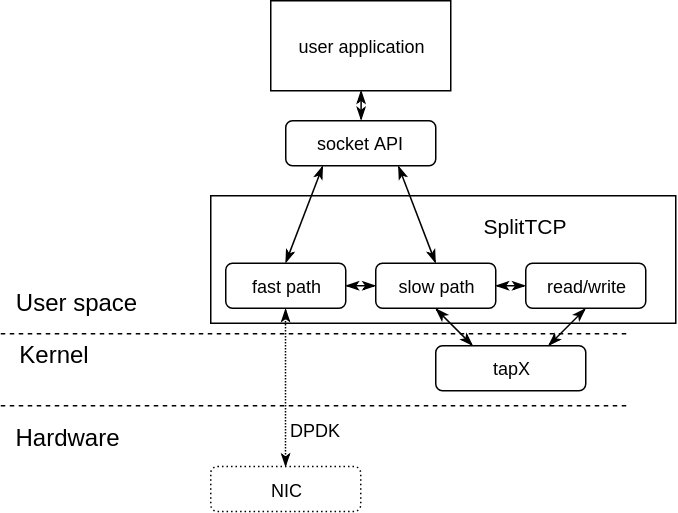
\includegraphics[width=\columnwidth]{figures/splittcp.png}
\caption{TBD.}
\label{fig:splittcp}
\end{figure}


* functionality glue

* Tap devices


\begin{figure}
\centering
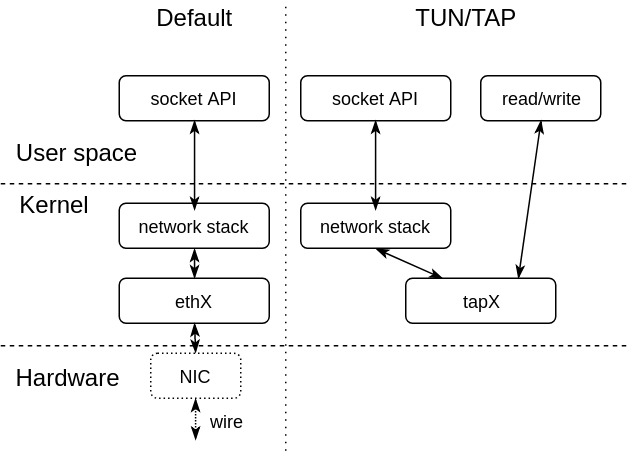
\includegraphics[width=\columnwidth]{figures/tap_diag.png}
\caption{TBD.}
\label{fig:tap}
\end{figure}
\section{Design}\label{Design}

\subsection{TAS Design}

TAS seeks to address a number of problems in the realm of datacenter packet
processing such as efficiency, predictability, and workload proportionality. 
Several important design decisions were made to accomplish these, but we will 
focus on just two of those: the split into a fast path and a slow path, and the
implementation of a userspace TCP stack.

One key way that TAS achieves high connection scalability and 
predictability is by dividing TCP functionality into two components: a fast 
path and a slow path. The fast path handles common-case packets and detects 
exceptions that need to be handled in the slow path. The main functions that
the fast path handles are common case send/receive, where the fast path directly
reads or writes packet payloads from application buffers and interacts directly
with the network, fast ACK handling, where the fast path will either generate or
consume ACK packets quickly without having to invoke the slow path, and 
efficient exception recognition and forwarding. 

In doing this, heavyweight TCP operations are taken out of the data path and 
relegated to the slow path, where they can be handled without affecting the 
performance of other flows in the fast path. The slow path does costly, 
infrequent operations like connection setup and teardown, timeouts, and 
enforcing congestion control. The slow path also handles out of order packets, 
but these are very infrequent in a datacenter environment.
   
In order for this separation and the individual components of the fast path 
and slow path to stay efficient, everything is implemented in a userspace TCP
stack. This provides all the normal functionality of TCP without having to 
switch back and forth between user and kernel space. This is good for 
performance and ease of programming, but isolates the TCP stack from Linux.
While we don't want to rely on Linux for performance operations, it does contain
information about the network and a configurability that would be useful in a 
datacenter environment.

\subsection{Integration Goals}

To most effectively interface with Linux, we take advantage of the previously 
described TAS design choices in order to minimize our impact on common case
packet processing. 

First, we don't make any modifications to the fast path code or data structures.
We prioritize making changes around the fast path, but add no additional lines 
of code to common case packet processing, and no additions and minimal 
interaction with fast path data structures to avoid incurring contention, cache 
problems, or race conditions. By following this rule, we shouldn't incur any
direct overheads to the cases that we care most about.

Secondly, we don't worry about performance in the slow path as long as it
doesn't incur any scheduling or blocking problems with the fast path. We have 
very little control over how often Linux will deliver packets to the slow path, 
so we want to make sure this doesn't negatively affect the fast path threads 
when they might be co-scheduled with the slow path.

\subsection{Compromises Made}

In order to accomplish these goals, we made some compromises to certain problems
in our implementation. In these cases, we could have used few lines of code or 
perhaps gotten better performance for the slow path operation, but at the 
expense of potentially slowing down the fast path.

First, as previously discussed, the fast path naturally consumes all ACK packet,
including during connection setup. In order to most faithfully setup the 
connection, we would need to modify the fast path to either forward ACK packets 
to the slow path, or write packets directly to the tap device. Instead of 
absorbing these costs in the fast path, we instead manually create a new ACK
packet during connection setup in the slow path and write it to the tap device.

Second, we maintain separate sequence numbers between Linux and TAS and 
between TAS and remote hosts. TAS immediately initializes fast path 
state upon receiving a \textit{SYN} packet and doesn't update it after that unless 
there's some kind of exception. Although this takes place in the slow path,
this would require adding some kind of complexity, as we won't know the sequence
number Linux wants to use until it provides a \textit{SYN/ACK}. We can address this by 
doing one of the following: adding an artificial delay or some kind of signal 
from the thread interacting with Linux in the middle of \textit{SYN} processing to make 
sure the sequence number is available when fast path state is initialized, 
initializing fast path state at a later time, modifying the fast path to 
identify either outgoing \textit{SYN/ACK} packets or incorrect outgoing sequence numbers
and adapting, or keeping separate sequence numbers. The final solution ended up 
being the simplest; the first will slow down connection setup even more, the 
second may create additional race conditions or problems in connection setup, 
and the last will slow down the fast path in some way.

Third, similarly to the first compromise, we handle ARP packets manually in 
the slow path, as they are not always forwarded to the slow path. By default,
the fast path only forwards ARP packets to the slow path if it is an IP address
that it doesn't have state for. As connection state is initialized immediately 
upon a \textit{SYN} packet being received, if we try to forward any Linux ARPs to the 
network for that connection, the replies will be dropped by the fast path. In
this case, instead of forwarding all ARP packets to the slow path or delaying
initializing connection state again, we fake ARP responses to Linux requests 
in the slow path by searching TAS's ARP table and manually crafting 
packets. 

\begin{figure}
\centering
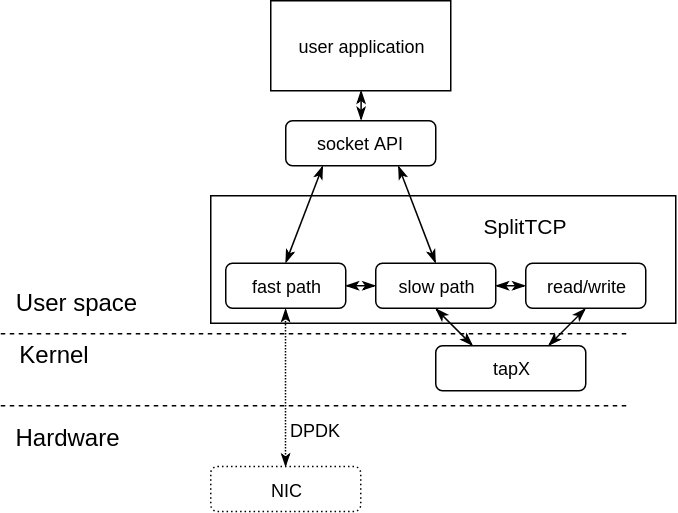
\includegraphics[width=0.7\columnwidth]{figures/splittcp.png}
\caption{Design of TAS with kernel integration. TAS now replicates all slow path operations to the kernel, checks what
it did by reading raw packets from the TAP device and mimics its decisions.}
\label{fig:splittcp_tap}
\end{figure}

\section{Implementation}\label{sec:impl}

We have implemented \taas from scratch in 10,127 lines of C code
(LoC). \taas' fast path comprises 2,931 LoC. The slow path comprises
3,744 LoC. The user-level library providing the POSIX sockets API is
dynamically linked to unmodified application binaries and comprises
3,452 LoC.

\paragraph{Fast path.}
The fast path runs in a user-level process, separate from the
applications. The fast path uses DPDK~\cite{dpdk} to directly access
the machine's NIC, bypassing the Linux kernel. Unlike systems that
rely on batching to reduce kernel-user switches, \taas uses a
configurable number of dedicated host cores, which we can vary based
on the offered network load. Each core replicates a linear packet
processing pipeline and exposes a queue pair to the slow path and to
each application context to avoid synchronization. The NIC's RSS
mechanism ensures that packets within flows are assigned to the same
pipeline and not reordered.

\paragraph{Slow path.} The slow path runs as a separate thread within
the fast process. To bootstrap context queues, we require applications
to first connect to the slow path via a named UNIX domain
socket. Applications use the socket to set up a shared memory region
for the context queues. The slow path also uses the socket for
automatic cleanup, to detect when application processes exit by
receiving a hangup signal via the corresponding socket.

\subsection{Limitations}

\paragraph{Fixed connection buffer sizes.}
\softtcp requires connection send and receive buffers to be fixed upon
connection creation. We do not currently implement any buffer resizing
depending on load.  For workloads with large numbers of inactive
connections, buffer resizing (via additional management commands) is
desirable.

\paragraph{TCP slow start.} Our prototype does not fully implement the
TCP slow start algorithm. Instead, we current double the sending rate
every RTT until we reach steady-state. Since our measurements are only
concerned with steady-state performance, this limitation does not
impact the reported results.

\section{Evaluation}\label{Eval}

In this section, we evaluate our implementation of Linux-Integrated TAS. Our
evalutation seeks to answer the following questions:

\begin{itemize}
    \item Do our changes affect the performance of the fast path?
    \item What is the performance of the slow path?
\end{itemize}

\subsection{Evaluation Setup}

To answer the above questions, we run a simple RPC echo server microbenchmark. A  
client sends a packet with a 64 byte payload to a server, which echos the packet
back to the client. Both client and server are single threaded. The server 
machine is an Intel Xeon Gold 6138 system at 2.0 GHz with a 1G NIC. The client 
machine is an Intel Xeon E3-1225 v3 system at 3.3 GHz with a 1G NIC. Both client 
and server run Linux kernel 4.18.

\subsection{Fast Path Performance}

\begin{table}[]
\begin{tabular}{@{}crrrrrr@{}}
\toprule
               & \multicolumn{6}{c}{Latency (us)}                                                                                                                                    \\ \midrule
               & \multicolumn{3}{c}{TAS}                                                          & \multicolumn{3}{c}{Linux-Integrated TAS}                                         \\
\# Connections & \multicolumn{1}{c}{Avg} & \multicolumn{1}{c}{99\%} & \multicolumn{1}{c}{99.99\%} & \multicolumn{1}{c}{Avg} & \multicolumn{1}{c}{99\%} & \multicolumn{1}{c}{99.99\%} \\
1              & 60                      & 70                       & 79                          & 61                      & 62                       & 78                          \\
2              & 63                      & 65                       & 97                          & 62                      & 64                       & 82                          \\
4              & 65                      & 68                       & 105                         & 65                      & 89                       & 118                         \\
8              & 71                      & 79                       & 147                         & 70                      & 78                       & 151                         \\
16             & 68                      & 77                       & 144                         & 69                      & 76                       & 146                         \\
32             & 72                      & 97                       & 170                         & 74                      & 104                      & 153                         \\ \bottomrule
\end{tabular}
\label{fastpath-latency}
\end{table}

Table \ref{fastpath-latency} shows the average and tail latencies of the RPC 
echo microbenchmark with TAS and Linux-Integrated TAS. The average-case latency
of the fast path of Linux-Integrated TAS is within 3\% of TAS. The performance 
at the tail varies a bit more between the two versions, but is within 25\% of 
TAS in the worst case.

Figure \ref{fig:fastpath-throughput} shows the throughput of the RPC echo server
microbenchmark using the original TAS and Linux-Integrated TAS. The throughput 
of both versions are very similar.

\paragraph{Discussion.} Our evaluation results show that the fast path 
performance of Linux-Integrated TAS is very similar to the fast path performance 
of the original TAS. This result aligns with the fact that we made no changes to
the fast path. Additionally, slow path operations such as connection setup and
teardown happen infrequently enough that they do not affect the performance of 
the fast path.

\begin{figure}
  \centering
  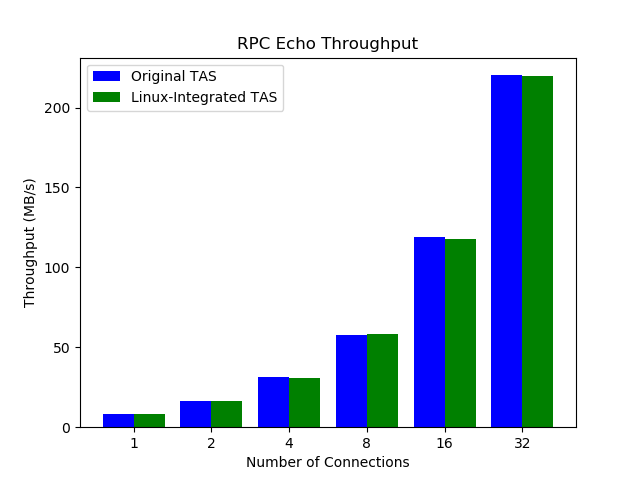
\includegraphics[width=\columnwidth]{figures/rpc_echo_throughput.png}
  \caption{RPC echo throughput for a single threaded client and server.}
  \label{fig:fastpath-throughput}
\end{figure}

\subsection{Slow Path Performance}

Our performance results show that the slow path performance is reduced 
drastically compared to the original TAS. Connection setup times were reported 
on the order of seconds. This is due to the fact that we now incur system call 
overheads on the slow path. We must wait for Linux to handle the packets we send 
to it before we can observe its response. For example, we must issue a blocking 
accept call to Linux to ensure that TAS does not prematurely move on to the next 
connection before observing Linux's response.
\section{Related Work}

% Data Center TCP (DCTCP), SIGCOMM 2010
% Misbehaving Receivers, CCR 1999
% Robust ECN Signalling with Nonces 
% https://www.cs.umd.edu/~nspring/talks/ietf-ecn.pdf
% \paragraph{Improvements to TCP.}
% The TCP protocol is constantly evolving, e.g., to improve TCP's attack
% resilience with nonces~\cite{misbehaving_receivers_ccr_1999}, to
% handle out of order packets more efficiently~\cite{juggler_eurosys16},
% to add better loss recovery mechanisms~\cite{aggression}, to improve
% congestion
% control~\cite{timely,dctcp,bbr,pcc,tcp_illinois,recursive_congestion,tcp_ex_machina,dcqcn},
% or to perform bandwidth allocation~\cite{numfabric,fastpass}. The key
% to adoption has been to keep the TCP packet format untouched. Our work
% is intended to be compatible with this line of work; \softtcp avoids
% binding protocol decisions into hardware.

\paragraph{Software TCP stack improvements.}
A closely related line of work aims to reduce TCP CPU overhead,
often with some level of NIC assistance; we push this farther by 
co-designing the NIC and software layers.
Many of these systems also use batching to reduce overhead at some cost in
latency; our focus is on reducing overhead for latency-sensitive RPCs 
where batching is less appropriate. 
Affinity-accept~\cite{affinity-accept} and Fastsocket~\cite{fastsocket} 
use flow steering on the NIC to keep connections local to cores. 
mTCP~\cite{mtcp} uses NIC virtualization to move the TCP stack
into each application, eliminating kernel calls in the common case,  
at the cost of trusting the application to implement congestion control.
Sandstorm~\cite{sandstorm} co-designs the TCP stack using 
application-specific knowledge about packet payloads; this is an interesting 
avenue for future work.
Megapipe~\cite{megapipe} re-designs the kernel-application interface 
around communication channels; we use a similar idea in our design. 
IX~\cite{belay:ix} pushes this farther by also changing the socket interface;
we aim to keep compatibility with existing applications.  To
improve load balancing, ZygOS~\cite{zygos} introduces an object steering 
layer that is similar to ours. Finally, CCP proposes separating congestion
control policy from its enforcement~\cite{ccp}; our work can be seen
as an implementation of that idea.

% Network stack redesigns:
% Scalable IP stacks using kernel bypass: mTCP (NSDI). Network stack specialization for performance (SIGCOMM'14).
% JUGGLER: A Practical Reordering Resilient Network Stack for
% Datacenters (EuroSys'16)
% Scalable TCP design for Linux (ASPLOS'16). affinity-accept. Megapipe.

Within a virtualized cloud context, NetKernel~\cite{netkernel} also
proposes to separate the network stack from guest OS kernels and to
offer it as a cloud service in a separate virtual machine. Unlike
\softtcp, NetKernel's goal is to allow cloud operators more control
over tenant network stacks and to accelerate provider-driven network
stack evolution by enabling new network protocol enhancements, such as
congestion control, and to make it available to all tenant VMs
transparently and simultaneously. \softtcp can provide the same
benefit, but our focus is on leveraging the separation of OS kernel
and network stack to streamline packet processing.

\paragraph{NIC-Software co-design.}
Previous attempts to improve packet processing performance used new
HW/SW interfaces to reduce the number of required PCIe transitions
\cite{flajslik:llnic,binkert:inic}, to scale rate
limiting~\cite{senic}, and to enable kernel-bypass
\cite{pratt:arsenic,voneicken:unet,druschel:osiris}. TCP Offload
Engines~\cite{toe,chelsio_toe} and remote direct memory access
(RDMA)~\cite{rdma} go a step further, entirely bypassing the remote
CPU for their specific use-case. Scale-out
NUMA~\cite{novakovic:sonuma} extends the RDMA approach by integrating
a remote memory access controller with the processor cache hierarchy
that automatically translates certain CPU memory accesses into remote
memory operations. Portals~\cite{portals_spec} is similar to RDMA, but
adds a set of offloadable memory and packet send operations triggered
upon matching packet arrival. Out of these approaches, only kernel
bypass has found broad market acceptance. One hindrance to widespread
adoption of network stack offload is that hardware stack deployment is
slower than software stack deployment, while application demands and
datacenter network deployments change rapidly. Hardware approaches are
thus often not able to keep pace fast enough with the changing world
around them. By providing an efficient software network stack,
\softtcp side-steps this issue, while providing performance close to
that of hardware solutions.

% An interesting future research direction
% is to show that the Portals model and \rmttcp can both be supported on
% the same configurable NIC hardware platform.

\section{Conclusion}

The continuing increase in data center link bandwidth, coupled with a
much slower improvement in CPU performance, is threatening the
viability of kernel software TCP processing, pushing researchers to
investigate alternative solutions. Any alternative has to ensure that
it is safe, efficient, scalable, and flexible.

We present \taas, TCP acceleration as a software service. \taas
executes common-case TCP operation in a linearized fast path, while
handling corner cases in a slow path.  \taas achieves throughput up to
4.5$\times$ that of Linux and up to 1.5$\times$ that of IX for common
cloud applications.
% A further 1.6 speedup is possible on some applications through
% object steering on the NIC.
Unlike kernel bypass, \taas enforces congestion control on untrusted
applications, and achieves much higher levels of per-flow fairness
than Linux. \taas scales to many cores and connections, while being
flexible to further TCP protocol innovation.


{\footnotesize
\bibliographystyle{acm}
\bibliography{paper,strings,defs}}

\end{document}
